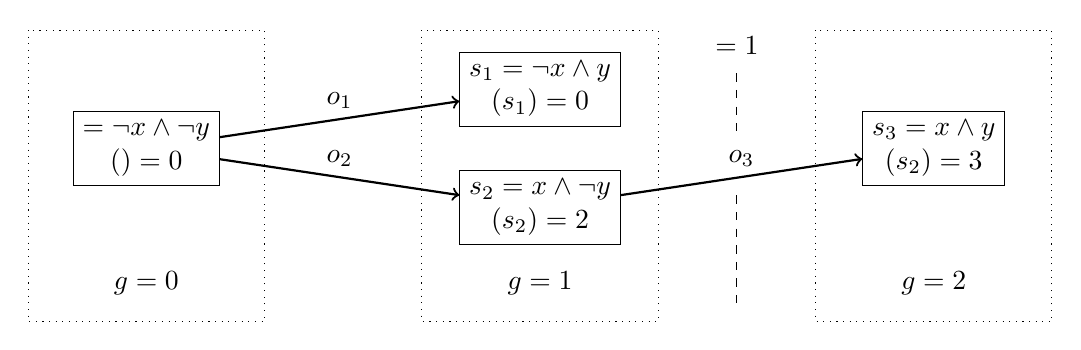
\begin{tikzpicture}[yscale=1]
    \begin{scope}
        \node[align=center,draw] (s0) at (0,0) {$\init = \lnot x \land \lnot y$\\$\utility(\init) = 0$};
        \node[align=center,draw] (s1) at (5,0.75) {$s_1 = \lnot x \land y$\\$\utility(s_1) = 0$};
        \node[align=center,draw] (s2) at (5,-0.75) {$s_2 = x \land \lnot y$\\$\utility(s_2) = 2$};
        \node[align=center,draw] (s3) at (10,0) {$s_3 = x \land y$\\$\utility(s_2) = 3$};

        \draw[dotted] (-1.5,1.5) rectangle (1.5,-2.2) node[pos=.5,align=center] {\\\\\\\\\\\\\\$g = 0$};
        \draw[dotted] (3.5,1.5) rectangle (6.5,-2.2) node[pos=.5,align=center] {\\\\\\\\\\\\\\$g = 1$};
        \draw[dotted] (8.5,1.5) rectangle (11.5,-2.2) node[pos=.5,align=center] {\\\\\\\\\\\\\\$g = 2$};

        \draw[dashed] (7.5,0.95) to (7.5,0.2);
        \draw[dashed] (7.5,-0.6) to (7.5,-2.0);
        \node[align=center] at (7.5,1.3) {$\limit = 1$};

        \draw[->, thick] (s0) to node [above, align=center] {$o_1$} (s1);
        \draw[->, thick] (s0) to node [above, align=center] {$o_2$} (s2);
        \draw[->, thick] (s2) to node [above, align=center] {$o_3$} (s3);
    \end{scope}
\end{tikzpicture}